\documentclass{uebblatt}

\newcommand{\http}{http:/\kern-.2em/\kern-0.03em}

\begin{document}

\maketitle{1}{Abgabe bis zum Montag, den 19. Oktober 2015 \\
Kummerkasten auf algebra.speicherleck.de}

\begin{aufgabe}{m+2+2}{Invertierbarkeit und Nilpotenz in Polynomringen}
Sei~$A$ ein Ring. Sei~$f = a_0 + a_1 X + \cdots + a_m X^m \in A[X]$ ein Polynom
über~$A$. Zeige:
\begin{enumerate}
\item Genau dann ist~$f$ eine Einheit in~$A[X]$, wenn~$a_0$ in~$A$ invertierbar
und die~$a_1,\ldots,a_m$ nilpotent sind.
\item Genau dann ist~$f$ nilpotent, wenn~$a_0,\ldots,a_m$ nilpotent sind.
\item Ist~$A$ \emph{reduziert}, d.\,h. ist nur die Null in~$A$ nilpotent,
und ist~$g = b_0 + \cdots + b_n X^n \in A[X]$ mit~$fg = 0$, so gilt für alle passenden Indizes~$i$ und~$j$: $a_i b_j = 0$.
\end{enumerate}
\end{aufgabe}

\begin{aufgabe}{2+m}{Lokale Ringe}
\begin{enumerate}
\item Zeige, dass ein Ring~$A$ genau dann lokal ist,
wenn~$1 \neq 0$ in~$A$ und, wann immer eine Summe aus zwei Elementen
invertierbar ist, schon ein Summand invertierbar ist.
\item Was sind die einzigen idempotenten Elemente in einem lokalen Ring?
\end{enumerate}
\end{aufgabe}

\begin{aufgabe}{4}{Ringe mit nur einem Primideal}
Sei~$A$ ein Ring. Sei~$\nnn$ das Ideal der nilpotenten Elemente in~$A$. Zeige, dass folgende
Aussagen äquivalent sind:
\begin{enumerate}
\item[1.] In~$A$ gibt es genau ein Primideal.
\item[2.] Jedes Element von~$A$ ist \emph{entweder} invertierbar \emph{oder}
nilpotent.
\item[3.] Der Faktorring~$A/\nnn$ ist ein Körper.
\end{enumerate}
{\scriptsize\emph{Hinweis.} Verwende für den Teil~"`1. $\Rightarrow$ 2."' ohne
Beweis folgendes Lemma, das nächste Woche in der Vorlesung bewiesen wird: Der
Schnitt über alle Primideale eines Rings besteht nur aus seinen nilpotenten
Elementen.\par}
\end{aufgabe}
\enlargethispage{1.8em}

\begin{aufgabe}{m+2+2+2}{Boolsche Ringe}
Sei~$A$ ein \emph{boolscher Ring}, d.\,h. ein kommutativer Ring mit~$x^2 =
x$ für alle~$x \in A$. Zeige:
\begin{enumerate}
\item Für alle~$x \in A$ gilt~$2x = 0$.
\item Jedes Primideal~$\ppp$ von~$A$ ist maximal.
\item Für jedes Primideal~$\ppp$ von~$A$ ist~$A/\ppp$ ein Körper mit zwei
Elementen.
\item Jedes endlich erzeugte Ideal von~$A$ ist ein Hauptideal.
\end{enumerate}
\end{aufgabe}

\vfill
\begin{center}
  \rotatebox{90}{\tiny\sffamily \http spikedmath.com/182.html}
  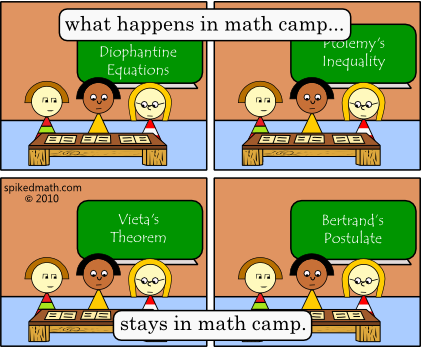
\includegraphics[height=3.7cm]{images/what-happens-in-math-camp}
\end{center}

\end{document}
